\chapter{Tempat Hewan Hidup}\label{ch:g2:where-animals-live}

Kamu tidak akan berjumpa ikan trout di halaman sekolah, dan juga tidak
akan berjumpa tupai di dasar kolam. Tiap \omterm{def:g1:animals-around-us:animal}{hewan} hidup di tempat yang
cocok baginya --- tempat ia menemukan makanannya, perlindungannya dan
tetangganya. Ahli \omterm{def:g1:living-or-not:living}{biologi} punya nama untuk tanah tempat tinggal seekor
\omterm{def:g1:animals-around-us:animal}{hewan}.

\section{Habitat}

\begin{definition}[Habitat]\label{def:g2:where-animals-live:habitat}
Yang disebut \emph{habitat}\index{habitat} seekor \omterm{def:g1:animals-around-us:animal}{hewan} adalah jenis
tempat yang secara alami dihuninya dan tempat ia menemukan segala yang
dibutuhkannya: makanan, air, perlindungan, dan tempat yang aman bagi
anaknya. Kolam, hutan, padang rumput, pagar tanaman dan tepi laut
adalah habitat.
\end{definition}

\begin{example}[Empat habitat, empat lingkungan]\label{ex:g2:where-animals-live:four}
Di \emph{kolam}: katak, capung, ikan duri, siput kolam. Di
\emph{hutan}: tupai, rusa, burung pelatuk, semut kayu. Di
\emph{padang rumput}: kelinci, belalang, kupu-kupu, tikus ladang. Di
bawah batu sebuah \emph{tembok} tua: kutu kayu, laba-laba, kadang
seekor kadal yang berjemur di atasnya.
\end{example}

\begin{omfigure}
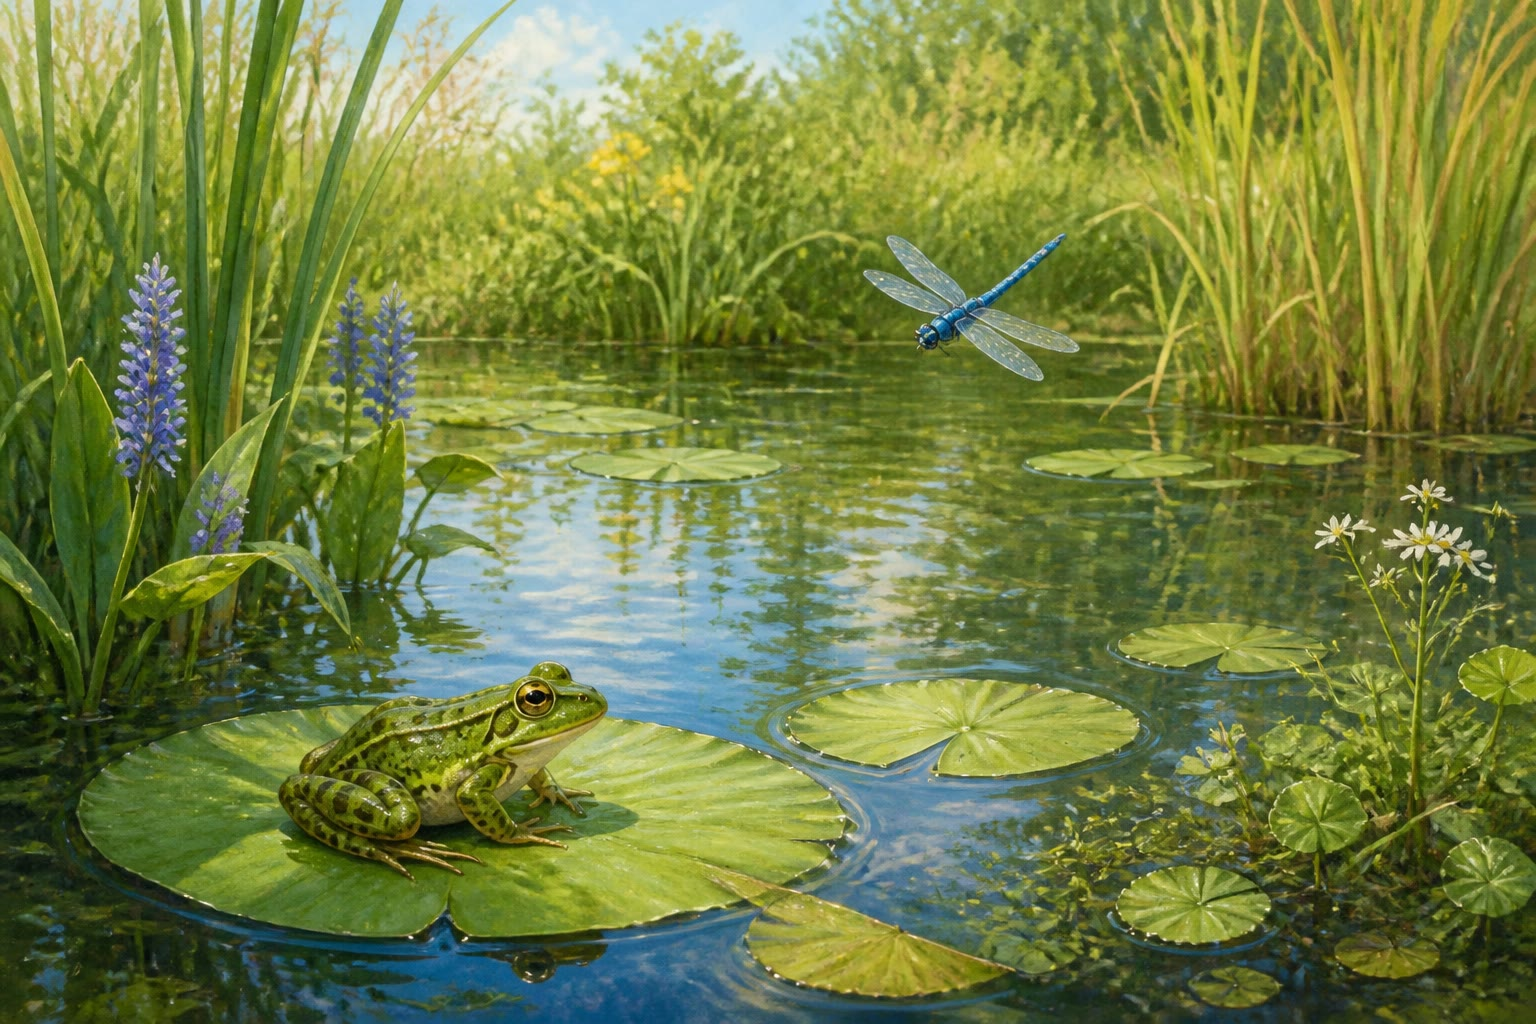
\includegraphics[width=0.62\linewidth]{images/book1/ai/g2-live-pond.jpg}

{\small \omterm{def:g2:where-animals-live:habitat}{Habitat} kolam bersama dua penghuninya di rumah: seekor katak
di atas \omterm{def:g1:plants-around-us:parts}{daun} teratai, seekor capung yang berpatroli.}
\end{omfigure}

\begin{omfigure}
\begin{tikzpicture}[scale=0.88]
  \draw[thick, omDef, fill=omDef!7, rounded corners=6pt]
    (0,0) rectangle (3.4,2.6);
  \draw[thick, omMeth, fill=omMeth!7, rounded corners=6pt]
    (3.9,0) rectangle (7.3,2.6);
  \draw[thick, omProp, fill=omProp!7, rounded corners=6pt]
    (7.8,0) rectangle (11.2,2.6);
  \node[font=\small\bfseries, omDef] at (1.7,2.25) {kolamnya};
  \node[font=\small\bfseries, omMeth] at (5.6,2.25) {hutannya};
  \node[font=\small\bfseries, omProp] at (9.5,2.25) {padang rumputnya};
  \node[font=\small, align=center] at (1.7,1.05)
    {katak\\ capung\\ ikan duri};
  \node[font=\small, align=center] at (5.6,1.05)
    {tupai\\ burung pelatuk\\ rusa};
  \node[font=\small, align=center] at (9.5,1.05)
    {kelinci\\ belalang\\ kupu-kupu};
\end{tikzpicture}

{\small Tiga \omterm{def:g2:where-animals-live:habitat}{habitat} dan sebagian penghuninya. Cobalah menukarnya ---
tupainya tidak akan bertahan lama di kolam.}
\end{omfigure}

\begin{remark}[Satu habitat, banyak rumah]\label{rem:g2:where-animals-live:layers}
Sebuah \omterm{def:g2:where-animals-live:habitat}{habitat} punya banyak sudut. Di dalam satu hutan, burung pelatuk
hidup tinggi di \omterm{def:g1:plants-around-us:parts}{batang} pohon, tupai di dahan, rusa di antara semak,
dan semut kayu di tanah dalam sarang gundukannya. Hutan yang sama,
lantai yang berbeda --- sehingga begitu banyak \omterm{def:g1:animals-around-us:animal}{hewan} dapat berbagi
satu \omterm{def:g2:where-animals-live:habitat}{habitat} tanpa berdesakan.
\end{remark}

\section{Terpasang untuk habitatnya}

\begin{proposition}[Hewan cocok dengan habitatnya]\label{prop:g2:where-animals-live:fit}
Tubuh dan kebiasaan seekor \omterm{def:g1:animals-around-us:animal}{hewan} cocok dengan tempat ia hidup:
\begin{itemize}
  \item kaki berselaput katak mendorong air --- dibuat untuk kolam;
  \item cakar pencengkeram tupai dan ekornya yang besar sebagai
        penyeimbang dibuat untuk pohon;
  \item kaki penggali kelinci dan \omterm{def:g1:the-five-senses:sense}{telinganya} yang panjang sebagai
        pemberi peringatan dibuat untuk padang rumput terbuka dengan
        liang di bawahnya;
  \item \omterm{def:g1:animals-around-us:covering}{bulu} bebek menolak air, dan kaki berselaputnya mengayuh.
\end{itemize}
Dipindahkan ke \omterm{def:g2:where-animals-live:habitat}{habitat} yang keliru, seekor \omterm{def:g1:animals-around-us:animal}{hewan} kehilangan semua
keunggulan ini.
\end{proposition}
\admitted

\begin{example}[Perlengkapan tikus tanah]\label{ex:g2:where-animals-live:mole}
Tikus tanah hidup di bawah tanah, dalam terowongan yang digalinya di
bawah padang rumput. Tangannya berupa sekop penggali yang lebar,
\omterm{def:g1:animals-around-us:covering}{bulunya} terbaring rata ke kedua arah sehingga tanah tidak pernah
mengacaknya, dan \omterm{def:g1:the-five-senses:sense}{matanya} yang lemah nyaris tidak berarti dalam gelap.
Di atas tanah ia kikuk; di dalam \omterm{def:g2:where-animals-live:habitat}{habitatnya} sendiri ia juara.
\end{example}

\begin{method}[Memasangkan hewan dengan habitatnya]\label{met:g2:where-animals-live:matching}
Diberikan seekor \omterm{def:g1:animals-around-us:animal}{hewan} yang belum dikenal:
\begin{enumerate}
  \item amati perlengkapannya: kaki berselaput? cakar? sayap? kaki
        penggali?
  \item tanyakan apa yang dimakannya, dan di mana makanan itu
        ditemukan;
  \item tanyakan di mana ia dapat berlindung dan membesarkan anaknya;
  \item \omterm{def:g2:where-animals-live:habitat}{habitat} yang menjawab ketiganya adalah rumahnya yang mungkin.
\end{enumerate}
\end{method}

\section{Habitat dapat hilang}

\begin{proposition}[Tanpa habitat, tanpa penghuni]\label{prop:g2:where-animals-live:loss}
Seekor \omterm{def:g1:animals-around-us:animal}{hewan} tidak dapat hidup tanpa \omterm{def:g2:where-animals-live:habitat}{habitatnya}. Kalau sebuah kolam
ditimbun, katak dan capungnya lenyap bersamanya; kalau sebuah pagar
tanaman dicabut, burung yang bersarang di situ kehilangan
perlindungannya. Melindungi \omterm{def:g1:animals-around-us:animal}{hewan} bermula dengan melindungi tempat
mereka hidup.
\end{proposition}
\admitted

\begin{example}[Kolam sekolah]\label{ex:g2:where-animals-live:schoolpond}
Sebuah sekolah menggali kolam kecil di sudut halamannya. Dalam dua
tahun, capung berpatroli di situ, anggang-anggang berjalan di
permukaannya, dan katak sudah pindah masuk --- tidak seorang pun
membawa mereka. Buatlah \omterm{def:g2:where-animals-live:habitat}{habitatnya}, dan penghuninya akan menemukannya.
\end{example}

\begin{remark}[Mengamati tanpa mengganggu]\label{rem:g2:where-animals-live:respect}
Ketika mengunjungi sebuah \omterm{def:g2:where-animals-live:habitat}{habitat}, kita adalah tamu. Amati dengan
tenang, kembalikan batu seperti keadaan semula, biarkan \omterm{def:g2:animals-grow-up:born}{telur} dan
sarang tidak tersentuh, dan bawa pulang sampahmu --- \omterm{def:g2:where-animals-live:habitat}{habitatnya}
seharusnya lupa bahwa kamu pernah di situ. Bab-bab berikutnya memberi
lebih banyak cara merawat alam.
\end{remark}

\section{Latihan}

\begin{exercise}[$\star$]\label{exo:g2:where-animals-live:1}
Apa itu \omterm{def:g2:where-animals-live:habitat}{habitat}? Sebutkan empat hal yang ditemukan seekor \omterm{def:g1:animals-around-us:animal}{hewan} di
dalamnya.
\end{exercise}

\begin{exercise}[$\star$]\label{exo:g2:where-animals-live:2}
Sebutkan dua \omterm{def:g1:animals-around-us:animal}{hewan} kolam, dua \omterm{def:g1:animals-around-us:animal}{hewan} hutan, dan dua \omterm{def:g1:animals-around-us:animal}{hewan} padang
rumput.
\end{exercise}

\begin{exercise}[$\star$]\label{exo:g2:where-animals-live:3}
\omterm{def:g2:where-animals-live:habitat}{Habitat} mana yang cocok untuk tiap \omterm{def:g1:animals-around-us:animal}{hewan}: ikan duri, burung pelatuk,
belalang, kutu kayu?
\end{exercise}

\begin{exercise}[$\star$]\label{exo:g2:where-animals-live:4}
Apa perlengkapan berenang katak? Dan apa perlengkapan memanjat pohon
milik tupai?
\end{exercise}

\begin{exercise}[$\star$]\label{exo:g2:where-animals-live:5}
Sebutkan tiga perlengkapan bawah tanah tikus tanah dari
\cref{ex:g2:where-animals-live:mole}.
\end{exercise}

\begin{exercise}[$\star$]\label{exo:g2:where-animals-live:6}
Pada \cref{rem:g2:where-animals-live:layers}, ``lantai'' hutan mana
yang dipakai tiap \omterm{def:g1:animals-around-us:animal}{hewan}: burung pelatuk, tupai, rusa, semut kayu?
\end{exercise}

\begin{exercise}[$\star$]\label{exo:g2:where-animals-live:7}
Apa yang terjadi pada katak dan capung ketika sebuah kolam ditimbun?
Apa yang diajarkannya tentang melindungi \omterm{def:g1:animals-around-us:animal}{hewan}?
\end{exercise}

\begin{exercise}[$\star$]\label{exo:g2:where-animals-live:8}
Cobalah: pilih satu \omterm{def:g2:where-animals-live:habitat}{habitat} kecil di dekatmu --- di bawah sebuah batu,
sebuah semak, sebuah petak \omterm{def:g1:plants-around-us:parts}{bunga}. Amati dengan tenang lalu daftarkan
setiap \omterm{def:g1:animals-around-us:animal}{hewan} yang kamu lihat dalam waktu yang tetap. Kembalikan tiap
batu ke tempatnya. Berapa banyak penghuni yang dimiliki \omterm{def:g2:where-animals-live:habitat}{habitat}
kecilmu?
\end{exercise}

\begin{exercise}[$\star\star$]\label{exo:g2:where-animals-live:9}
Seekor \omterm{def:g1:animals-around-us:animal}{hewan} misteri berkaki selaput, berbulu lebat yang menolak air,
dan berparuh pipih untuk menyaring. Pakai
\cref{met:g2:where-animals-live:matching} untuk menyebutkan
\omterm{def:g2:where-animals-live:habitat}{habitatnya} --- dan barangkali \omterm{def:g1:animals-around-us:animal}{hewannya}.
\end{exercise}

\begin{exercise}[$\star\star$]\label{exo:g2:where-animals-live:10}
Tomi ingin ``menolong'' seekor katak dengan membawanya pulang ke
sebuah terarium kering yang penuh makanan. Dengan memakai
\cref{prop:g2:where-animals-live:fit} dan
\cref{prop:g2:where-animals-live:loss}, jelaskan mengapa hal ini sama
sekali tidak akan menolong kataknya.
\end{exercise}
